%%%%%%%%%%%%%%%%%%%%%%%%%%%%%%%%%%%%%%%%%%%%%%%%%%%
% DECLARATION DE LA CLASSE DU DOCUMENT
%%%%%%%%%%%%%%%%%%%%%%%%%%%%%%%%%%%%%%%%%%%%%%%%%%%
%% Utiliser le format suivant:
% \documentclass[type de papier% ("letterpaper" demandé)
% , simple ou recto verso% ("oneside" ou "twoside")%
% , taille de la police% ("12pt" demandé)%
% , type de document% ("these", "memoire", "memoireprojet" ou "thesepararticles")%
% , langue du document ("francais" ou "english")%
% , options supplémentaires% ("creativecommons" pour préciser que le document est soumis à la licence créative commomns, "hyperref", "withAlgo2e" pour utiliser le package algorithm2e avec la mise en page correcte de la liste des algorithmes)
%]{thETS}

%% Exemple pour une thèse creative commons, utilisant le package hyperref
\documentclass[letterpaper%
,oneside%
,12pt%
,report%
,french
,hyperref
,withAlgo2e%
,final
]{thETS}

\usepackage{filecontents,pgfplots}
\usepackage{siunitx}
\pgfplotsset{compat=1.15}
\usepackage[export]{adjustbox}
\usepackage{multirow}
\usepackage{usebib}
\usepackage{pdflscape}
\usepackage{rotating}
\usepackage{enumitem}
\usepackage{hyperref}

% \usepackage[obeyFinal]{todonotes}

\newbibfield{quote}
% \bibinput{logiciel}
\bibinput{Robots}


\newcommand{\footcite}[1]{\footnote{\cite{#1}}}

%%%%%%%%%%%%%%%%%%%%%%%%%%%%%%%%%%%%%%%%%%%%%%%%%%%
% IMPORTANT: NOTES D'IMPRESSION POUR RESPECTER LES MARGES
%%%%%%%%%%%%%%%%%%%%%%%%%%%%%%%%%%%%%%%%%%%%%%%%%%%
%%  Si vous créez un fichier PDF directement avec PDFLatex, et vous utilisez Acrobat Reader
%% pour faire l'impression, n'oubliez-pas de changer l'option <<Mise à l'échelle>> pour la valeur
%% <<Aucune>> pour que les marges soient imprimés correctement.
%%%%%%%%%%%%%%%%%%%%%%%%%%%%%%%%%%%%%%%%%%%%%%%%%%%


%%%%%%%%%%%%%%%%%%%%%%%%%%%%%%%%%%%%%%%%%%%%%%%%%%%
% DECLARATION D'UNE LISTE DE RÉFÉRENCES SUPPLÉMENTAIRE
%%%%%%%%%%%%%%%%%%%%%%%%%%%%%%%%%%%%%%%%%%%%%%%%%%%
%% Exemple de création d'une liste de références en plus de la liste bibliographique
% "refs" est utilisé en suffixe des commandes de citation de de bibliogtraphie
%\newcites{refs}{LISTE DE RÉFÉRENCES}

%%%%%%%%%%%%%%%%%%%%%%%%%%%%%%%%%%%%%%%%%%%%%%%%%%%
% DECLARATION DES INFORMATIONS DE LA PAGE TITRE
%%%%%%%%%%%%%%%%%%%%%%%%%%%%%%%%%%%%%%%%%%%%%%%%%%%

\title{Conception et implémentation du contrôle pour le manipulateur d'une plateforme robotique mobile}

%% Chapitre 1-3
\author{Alexandre FRANCOEUR}
\coauthors{}
% \coauthors{Marc-Olivier BÉLISLE\\Charles GIGUÈRE\\Ludovic VANASSE}

%\reporttype{Chapitre 1: Description de la problématique}
% \reporttype{Chapitre 2: Cadre d'analyse}
\teacher{Vincent DUCHAINE}

\reporttype{Rapport technique élaboré dans le cadre du cours projets spéciaux GPA791}


\datedepot{7 AVRIL 2020}
%\datesoutenance{``Date de soutenance''}

%\directeur{M.}{Prénom Nom}{Nom du département et institution}

%\directeur{Mme.}{Prénom Nom}{Nom du département et institution}

%\codirecteur{Mme.}{Prénom Nom}{département et institution}

%\codirecteurB{M.}{Prénom Nom}{département et institution}

%\president{M.}{Prénom Nom}{département et institution}

%\examinexterne{M.}{Prénom Nom}{département et institution}{}

%\jury{Mme.}{Prénom Nom}{département et institution}{}

%%%%%%%%%%%%%%%%%%%%%%%%%%%%%%%%%%%%%%%%%%%%%%%%%%%
% CHANGEMENT DE L'INTITULÉ DU DIPLOME
%%%%%%%%%%%%%%%%%%%%%%%%%%%%%%%%%%%%%%%%%%%%%%%%%%%
%% Il est possible de modifier l'intitulé du diplome en redéfinissant la commande
% \lediplome, comme dans l'exemple suivant:
%\renewcommand{\lediplome}{DE LA MAÎTRISE\\AVEC MEMOIRE EN GÉNIE ÉLECTRIQUE\\M. Sc. A.}

%\listfiles

%%%%%%%%%%%%%%%%%%%%%%%%%%%%%%%%%%%%%%%%%%%%%%%%%%%
% DÉBUT DU DOCUMENT
%%%%%%%%%%%%%%%%%%%%%%%%%%%%%%%%%%%%%%%%%%%%%%%%%%%
\begin{document}

\pagenumbering{Roman}

%%- Affichage de la page titre -%%
\maketitle

% %%- Affichage de la présentatiton du jury -%%
% \presentjury

% %%%- Avant propos -%%
% \begin{avantpropos}

% \lipsum[1] % Texte de remplissage pour donner un exemple de la mise en page

% \end{avantpropos}



% %%- Remerciements -%%
% \begin{remerciements}
% \lipsum[1] % Texte de remplissage pour donner un exemple de la mise en page
% % \input{Texte/remerciements.tex}
% \end{remerciements}


% %%- Sommaire -%%

% \begin{sommaire}{Robotique, Contrôle, ROS, Cinématique inverse, USAR}
% \input{Texte/resume.tex}
% \end{sommaire}


% %%- Abstract -%%
% \begin{abstract}{Titre en anglais}{keyword1, keyword2}

% \lipsum[1] % Texte de remplissage pour donner un exemple de la mise en page

% \end{abstract}

%\listoftodos
%%- Affichage de la table des matières -%%
\tableofcontents


%%- Affichage de la liste des tableaux -%%
% \listoftables

%%- Affichage de la liste des Figures -%%
\listoffigures

%%- Déclaration et affichage de la liste des abbréviations -%%
\begin{listofabbr}[3cm]
% \item [IMU] Inertial measurement unit
% \item [LiDAR] Light Detection and Ranging
\item [NIST] National Institute of Standards and Technology\footnote{\href{https://www.nist.gov/el/intelligent-systems-division-73500/standard-test-methods-response-robots}{https://www.nist.gov}}
\item [ROS] Robot Operating System\footnote{\url{https://www.ros.org/}}
\item [SDF] Semantic Description Format\footnote{\url{http://sdformat.org/}}
\item [TORK] Tokyo Opensource Robotics Kyokai Association\footnote{\url{https://opensource-robotics.tokyo.jp/?lang=en}}
\item [UI] Interface utilisateur
\item [URDF]  Unified Robot Description Format\footnote{\url{http://wiki.ros.org/urdf}}
\item [USAR] Urban Search and Rescue
\end{listofabbr}

% %%- Déclaration et affichage de la liste des symboles -%%
% \begin{listofsymbols}[3cm]
% \item [a] Première lettre de l'alphabet
% \item [A] Première lettre de l'alphabet en majuscule
% \end{listofsymbols}


% \cleardoublepage

\pagenumbering{arabic}

% Marginpar à gauche du document
%\reversemarginpar

%%%%%%%%%%%%%%%%%%%%%%%%%%%%%%%%%%%%%%%%%%%%%%%%%%%
% EXEMPLE DE CORPS DE THÈSE OU MÉMOIRE
%%%%%%%%%%%%%%%%%%%%%%%%%%%%%%%%%%%%%%%%%%%%%%%%%%%

\begin{introduction}
% Le club
Le club Capra conçoit et fabrique des robots terrestres depuis ses débuts en 1998. En 2017, le club était à la recherche d'un nouveau défi. 
% La compétition
Suite à plusieurs recherches et discussions, il fut décidé que le club participerait à la compétition RoboCup Rescue. La RoboCup Rescue a pour mission de stimuler la recherche et le développement de robots pour la recherche et sauvetage en milieu urbain\footnote{Traduit de l'anglais: «Urban Search and Rescue (USAR)»}. Les épreuves de la compétition sont basées principalement sur les normes d'essais développées par l'organisme de standardisation américain «National Institute of Standards and Technology» (NIST)\footnote{\cite{jacoff_guide_2014}}.

% Le robot 2020
Nous sommes présentement en cours de conception de notre deuxième prototype pour cette compétition. Il est conçu pour être plus robuste et plus performant que le prototype précédent. Celui-ci adopte une géométrie similaire à celle des robots actuellement disponible sur le marché, soit quatre chenilles motrices pouvant être inclinées en fonction des besoins. À l'annexe \ref{annexe:inspirationRobots}, se trouvent des images de certains robots qui ont servi d'inspiration.

% Exemple de déclaration de figure
\begin{figure}
    \centering % Les figures doivent être centrées
    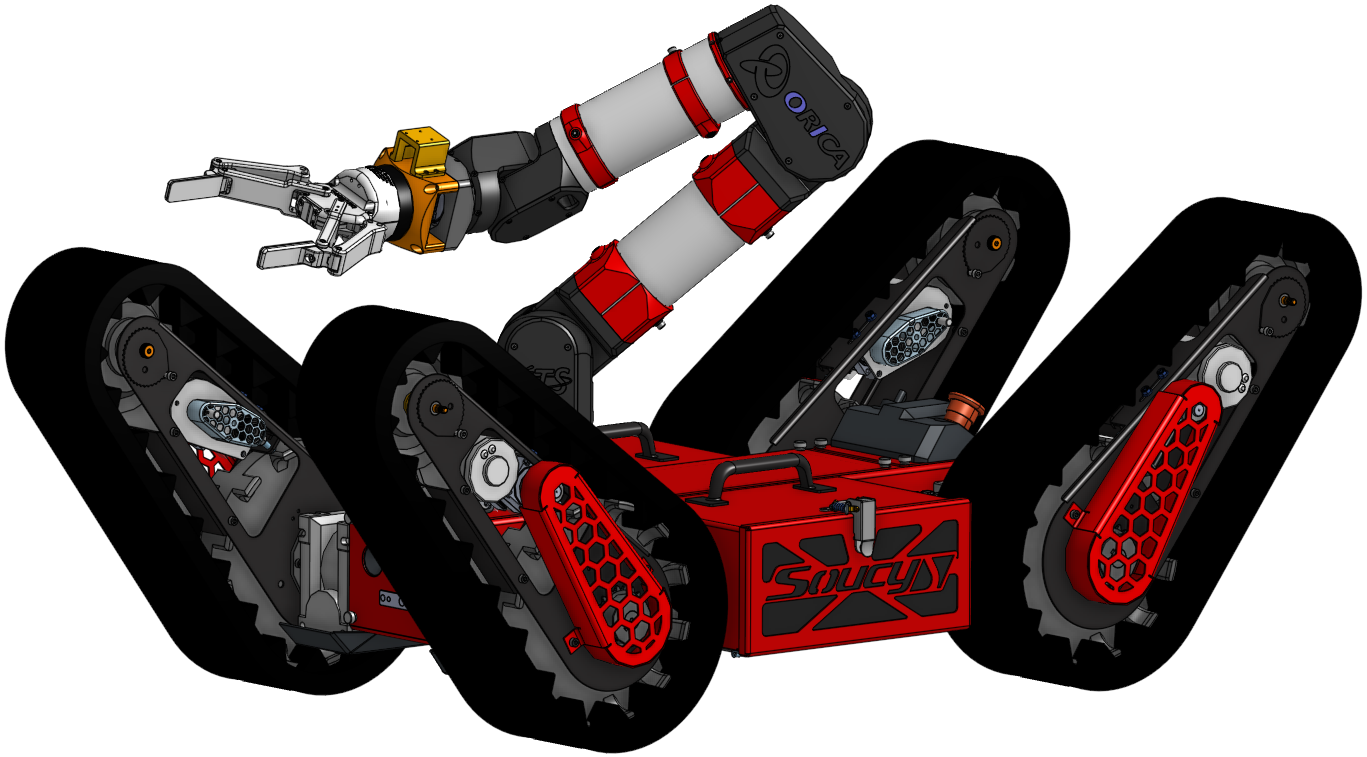
\includegraphics[width=0.85\textwidth]{Figures/markhor_ovis_cad.png}
    % \\ \parbox{0.75\textwidth}{
    \caption{La plateforme robotique Markhor équipée du bras robotique Ovis}
    \label{fig:markhor_ovis_CAD}
    % } % Utilisation d'une parbox pour restreindre la largeur de la légende. Ici la taille maximale a été fixée à la largeur choisie pour l'image (0.75\textwidth). Le décanat demande d'éviter d'avoir des légendes qui dépasse les figures, dans la mesure du possible (si l'image est trop petite, la légende peut dépasser sa largeur).
\end{figure}

Le sujet traité par ce rapport est le contrôle du bras manipulateur qui est attaché à la plateforme robotique. Pour ce faire, la problématique sera décrite puis analysée afin de définir l'objectif, l'objectif sera posé, les contraintes technologiques seront énoncés puis la mise en oeuvre de la solution sera décrite.

\end{introduction}

%\setcounter{chapter}{1}
\chapter{Description de la problématique}\label{chap:description}
\section{Mise en contexte}
Les services d'urgence sont appelés à travailler dans des conditions extrêmes. Dans le but de réduire leur exposition à certain types de danger tel que les radiations, sols instables, températures élevées, explosifs, ceux-ci utilisent des robots. L'utilisation de robots permet aux répondants de rester à une distance sécuritaire du danger. Toutefois, le temps de réponse et l'efficacité d'une intervention dépendent principalement des deux variables suivantes soit l'aisance de contrôle et la capacité pour l'opérateur à visualiser l'environnement qui entoure le robot.\footnote{\cite{massey_improved_2009}}

Par conséquent, le contrôle du robot devra être conçu de manière à être intuitif. Ceci dans le but de permettre à un opérateur n'ayant aucune expérience préalable, de maîtriser le bras robotique très rapidement. Poursuivant l'idée explorée par la marine américaine pour le contrôle du périscope de leurs sous-marins\footcite{brock_vergakis_navys_2017}, nous allons utiliser du matériel pré-existant et facile d'utilisation. Le but d'utiliser un composant en vente libre est qu'en raison des chaînes d'approvisionnement globales, il est possible de se procurer et de remplacer rapidement le matériel peu importe l'emplacement géographique où se déroule la mission.

Il n'y aura pas d'étude visant à qualifier la charge cognitive résultante de ce projet. Ceci parce que selon nos recherches, il n'existe pas à l'heure actuelle de méthode permettant de mesurer avec précision la charge mentale imposée à un opérateur. Certaines méthodes d'analyses existent tel que le NASA Task Load Index\footcite{hart_nasa_1986} mais celle-ci n'est pas en mesure de réduire suffisamment le biais du répondant. Une autre méthode qui semble plus probante est la mesure par oculométrie\footcite{st-onges_equipes_robots_2020} mais nous ne l'aborderons pas dans ce rapport étant donné que ce n'est pas le sujet de ce projet.

% \subsection{Requis de conception}
% \begin{enumerate}[align=left]
%     \item [\emph{Autonomous Flippers}] La compétition offre un multiplicateur
%     supplémentaire si les "flippers" se contrôlent sans une action de l'opérateur. Ceux-ci doivent être contrôlée selon des instructions strictes énoncés dans le cahier des règles de la compétition.\footcite{}
%     \item [\emph{Le robot doit pouvoir reculer}] Pour certains parcours de la compétition (MAN), le robot doit effectuer l'aller-retour sans pivoter sur lui-même.
% \end{enumerate}



% \section{Clients}
% \input{Texte/clients.tex}

% \section{Besoins}
% \input{Texte/besoins.tex}

% \section{Défauts et lacunes}
% \subsection{Défauts}
% \input{Texte/defauts.tex}

% \subsection{Lacunes}
% \input{Texte/lacune.tex}


\chapter{Dextérité: contrôle du bras robotique Ovis}
\label{chap:dexterity}

\section{Définition de l'objectif}
% Voir objectif SMART https://fr.wikipedia.org/wiki/Objectifs_et_indicateurs_SMART
\begin{figure}
    \centering % Les figures doivent être centrées
    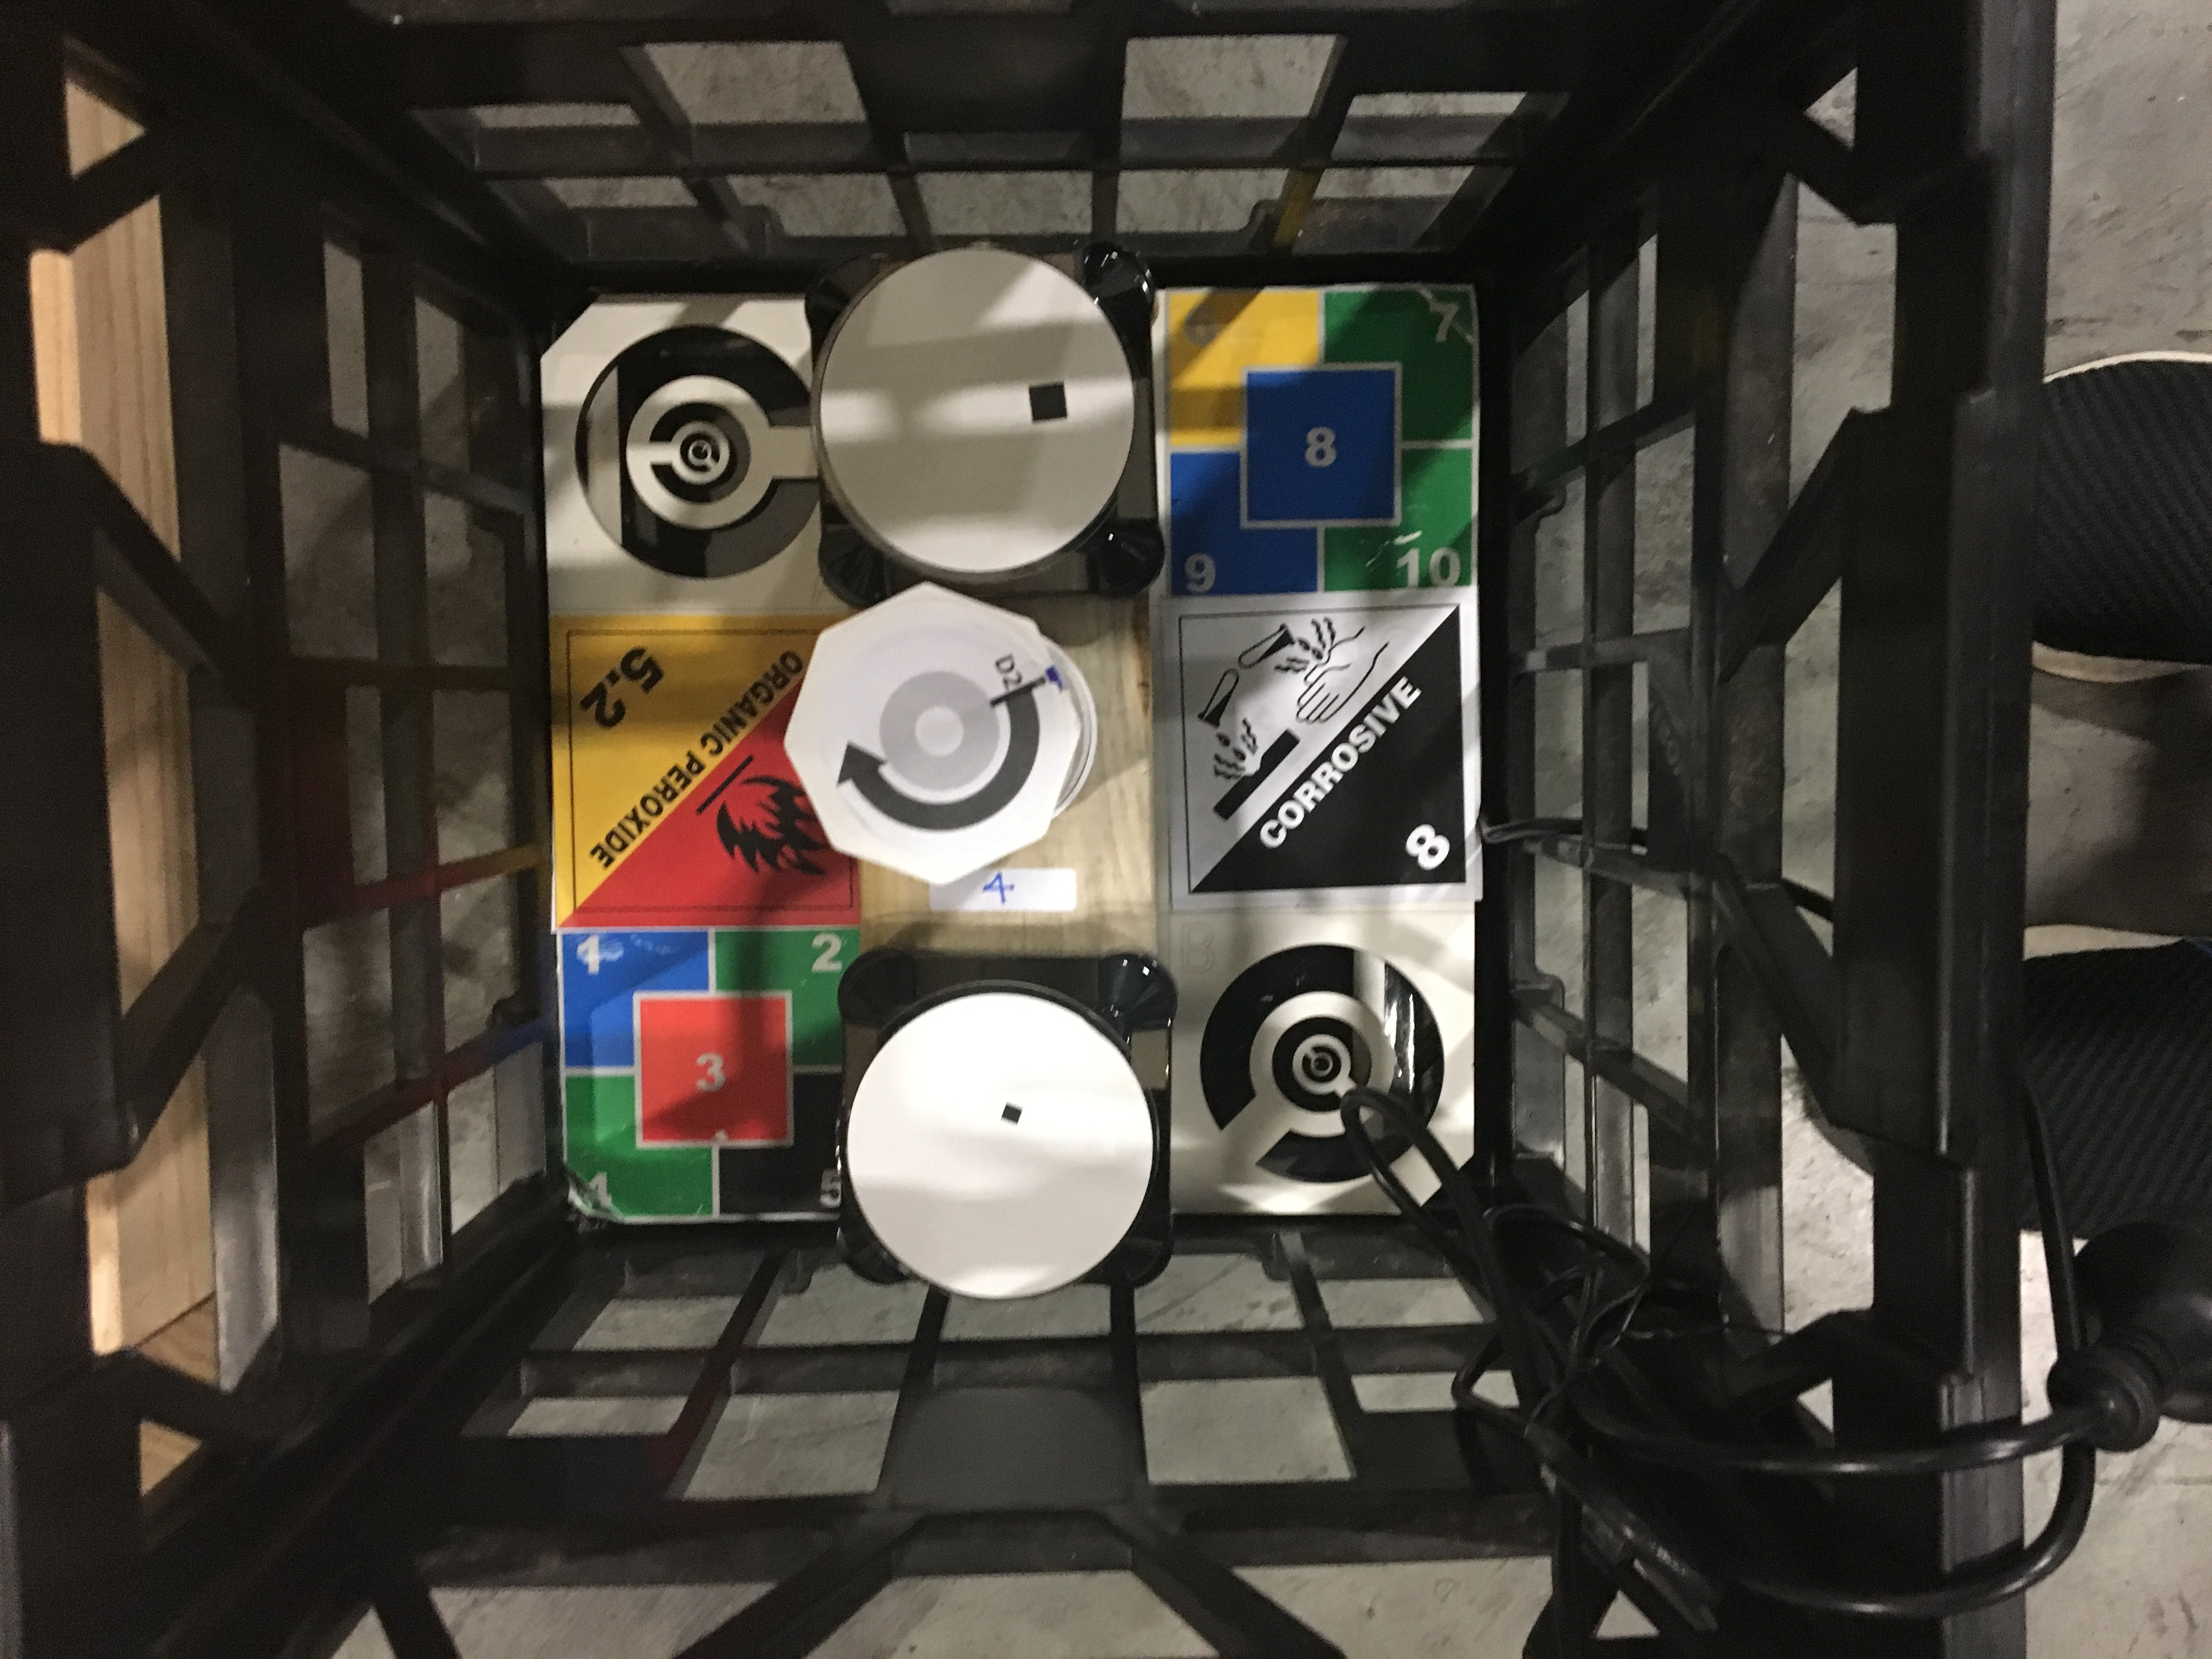
\includegraphics[width=0.75\textwidth]{Figures/test_method_rrl.JPG}
    \caption{Méthode d'essais de la RoboCup Rescue}
    \label{fig:test_method_rrl}
\end{figure}

L'objectif est de contrôler le bras robotique à l'aide d'instructions de mouvement cartésien. 
Le bras devra tenir compte de l'environnement qui l'entoure afin d'éviter une collision. La méthode d'essais qui sera utilisé à la RoboCup Rescue consiste à faire pivoter un tube de plastique PVC de 180 degrés puis de le retirer dans l'axe d'un autre tube de plus gros diamètre, le tuyau doit ensuite être déposé dans la caisse de lait. La figure \ref{fig:test_method_rrl} montre le banc d'essais qui met à l'épreuve les robots sur leur capacité à interagir avec les éléments de leur environnement. 
En ajout à l'objectif principal, on définira l'objectif plus ambitieux de contrôler le bras robotique à l'aide d'une souris 3D. La pince devra aussi être contrôlable en position, la vitesse d'ouverture/fermeture ainsi que la force de préhension seront contrôlables par les paramètres de l'interface utilisateur (UI) pour le moment.



\section{Choix technologiques}
\subsection{Matériel}
Le matériel suivant est déjà en possession du club Capra:
\begin{enumerate}[nosep]
    \item Actuateurs et contrôleur de Kinova
    \item Pince 2 doigts 140 mm de Robotiq
    \item Bras robotique Ovis
    \item Souris 3D - SpaceMouse de 3Dconnection
    \item Ordinateur embarqué - Nvidia Jetson Xavier%\footnote{\href{https://developer.nvidia.com/embedded/jetson-agx-xavier-developer-kit}{developer.nvidia.com/embedded/jetson-agx-xavier-developer-kit}}
\end{enumerate}

\subsection{Logiciel}
Les solutions logicielles suivantes sont présentement utilisées par le club Capra:
\begin{enumerate}[nosep]
    \item Ubuntu 18.04 LTS
    \item ROS Melodic Morenia%\footnote{\href{https://www.ros.org/}{ROS.org}}
    \item Interface utilisateur \href{https://github.com/clubcapra/capra_web_ui}{capra\_web\_ui} qui fonctionne sur Windows
\end{enumerate}
Les solutions logicielles suivantes seront explorées au cours de ce projet:
\begin{enumerate}[nosep]
    \item MoveIt\footcite{ioan_a_sucan_moveit_nodate}
    \item jog\_control\footcite{ryosuke_tajima_jog_control_nodate}
    \item kinova\_ros\textbackslash kinova\_driver
    \item Simulateur robotique Gazebo
    \item ROS industrial\_robot\_simulator
\end{enumerate}

\section{Implémentation}
\subsection{Description du robot}
La première étape de la programmation du bras robotique consiste à formuler la description (URDF). Cette description contient les éléments suivants:
\begin{itemize}
    \item L'origine et l'orientation des liens;
    \item La nature et les limites des axes;
    \item Les relations entre les liens et les axes;
    \item Les descriptions géométriques pour l'affichage et le calcul des collisions.
\end{itemize}

Une fois cette description écrite et validée, il est possible de générer une description plus complexe (SDF) à l'aide de l'assistant de configuration MoveIt. 

\subsection{Génération du paquet de support pour MoveIt}
L'assistant est simple à utiliser, il suffit de suivre les étapes énoncées dans le tutoriel, puis l'assistant génère un paquet de support utilisable par MoveIt.

Deux options s'offrent maintenant, simuler à l'aide du simulateur industriel ou simuler à l'aide du logiciel Gazebo. Ce dernier étant complexe à configurer et plutôt demandant en ressources, la première approche fut choisi afin d'effectuer des essais préliminaires.

\subsubsection{Génération du module d'extension IKFast}
La génération du module IKFast pour MoveIt requiert l'installation de la librairie OpenRave. La procédure d'installation et de configuration étant ardue, l'utilisation d'une image docker pré-configurée simplifie grandement la tâche. Le tutoriel MoveIt sur la création du module IKFast\footnote{\href{https://ros-planning.github.io/moveit_tutorials/doc/ikfast/ikfast_tutorial.html}{ros-planning.github.io/moveit\_tutorials/doc/ikfast/ikfast\_tutorial.html}} est précis, il suffit de suivre les instructions. Le seul problème rencontré est lors de la configuration des permissions, le tutoriel dit de fermer la session et de se reconnecter, ce n'était pas suffisant, un redémarrage est nécessaire.

\subsection{Simulation avec le simulateur industriel}
La configuration requise afin de simuler le bras robotique à l'aide du simulateur industriel n'est pas évidente à réaliser. Principalement parce que la documentation n'a pas suivi les mises à jour. En s'inspirant de la configuration d'autres manipulateurs industriels, il fut possible d'arriver au résultat visé.

\begin{figure}[H]
    \centering
    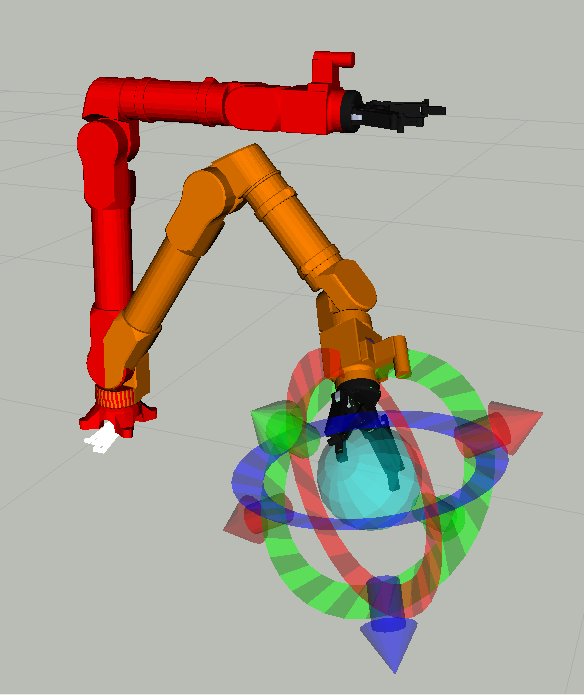
\includegraphics[scale=0.5]{Figures/ovis_moveit_industrial_sim}
    \caption{Ovis simulé par le simulateur industriel}
    \label{fig:ovis_industrial_sim}
\end{figure}

Sur la figure \ref{fig:ovis_industrial_sim}, on voit la position actuelle simulée (rouge), la position à atteindre simulée (orange) ainsi que le marqueur interactif (sphère cyan). Toutefois, on remarque que les joints de la pince robotique ne sont pas contrôlés (blanc). Ceci est dû à la lacune suivante du simulateur industriel. Le simulateur industriel est conçu pour un seul manipulateur, il n'émule donc pas plus d'un contrôleur logiciel. Les doigts de la pince ne sont pas localisés dans l'espace et se retrouvent affichée par défaut à la base du manipulateur.

\subsection{Simulation avec Gazebo}
En raison des lacunes que présente le simulateur industriel, il fut décidé que pour la suite du projet, il serait préférable de configurer la simulation Gazebo. Pour configurer la simulation Gazebo, il est possible d'utiliser le \emph{MoveIt Setup Assistant}, celui-ci génère un fichier URDF de base compatible avec Gazebo. Toutefois, ce fichier n'est pas modulaire et donc plus difficile à modifier et entretenir à l'avenir. Il fut donc décidé de continuer l'approche modulaire et d'étendre le contenu de la définition Xacro\footnote{\href{http://wiki.ros.org/xacro}{wiki.ros.org/xacro}} afin d'y inclure les paramètres spécifique à Gazebo tel que l'inertie, l'emplacement des capteurs de force et de la caméra du poignet. Il est aussi nécessaire d'ajouter le \emph{plugin} pour simuler le contrôleur logiciel du robot.

% \subsubsection{Abandon de la simulation Gazebo}
% Étant donné qu'il est complexe de modèliser le système et ne pouvant pas confirmer la validité de la simulation avec le bras réel, il fut décidé d'abandonner l'effort de simulation. Les efforts seront plutôt concentrés sur l'inter-connexion entre le logiciel et le matériel.

\subsection{Implémentation du contrôle linéaire}
La beauté de l'écosystème ROS est bien entendu sa communauté vouée à la recherche et au développement de la robotique. Il est souvent aisé de trouver une entité qui à dû traiter un problème identique ou similaire et qui publie sa solution librement. En cherchant une solution pour le déplacement linéaire d'un robot manipulateur, on a trouvé que le Tokyo Opensource Robotics Kyokai (TORK) avait déjà travaillé sur cette problématique. Leur solution \emph{jog\_control} étant librement accessible, il a donc suffit d'adapter le fichier de lancement de cette suite logicielle afin de la faire interagir avec le manipulateur.

\subsubsection{Contrôle du manipulateur à l'aide de la souris 3D}
\begin{figure}
    \centering
    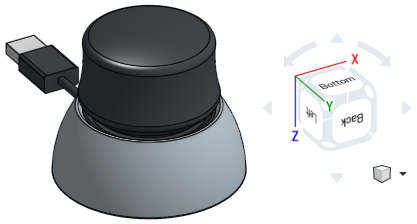
\includegraphics[width=0.65\textwidth]{Figures/spacemouse_axis_4.png}
    \caption{Le système d'axes de la souris 3D}
    \label{fig:spacemouse_axis}
\end{figure}

Le logiciel \emph{jog\_control} contenait déjà un exemple permettant de contrôler un manipulateur à l'aide d'une manette de jeux videos. L'exemple fut testé à l'aide d'une manette Xbox afin de valider qu'il était fonctionnel. Par la suite, l'adaptation avec la souris 3D fut entreprise. L'exemple étant écrit en python, le prototype d'adaptation pour le contrôle avec la souris 3D l'est aussi. Ayant en tête le projet actuel, ce travail fut effectué à la session A2019\footnote{\href{https://github.com/tork-a/jog_control/commit/b1b27c9a034a166a8e04d271c7839f4741c848b4}{github.com/tork-a/jog\_control@b1b27c9}}. Le prototype calcule d'abord une multiplication matricielle afin de passer des axes de la souris 3D tel que montrés à la figure \ref{fig:spacemouse_axis} vers le référentiel local à l'effecteur. 

% Après des essais plus exhaustif, il semblerait qu'il y ait une erreur de logique dans le prototype. Ce dernier permet les déplacement seulement vers la borne positive d'un axe, le problème semble se situer à la fonction du mode dominant. Celle-ci filtre le tableau des axes et conserve seulement la valeur la plus élevée.

La réécriture complète du logiciel fut débutée. Cette fois-ci, le logiciel est écrit en C++ afin d'augmenter la rapidité d'exécution. La réécriture comprend aussi un remodelage des différentes fonctions et variables membre de la classe. La réécriture ne fut pas sans heurt, la librairie ROS pour le C++ est plus complexe que celle pour python. Il fallut aussi trouver une librairie afin d'effectuer les calculs matriciels nécessaires pour le calcul des rotations, la librairie Armadillo\footcite{sanderson_armadillo_2016} fut sélectionné en raison de sa documentation exhaustive et de sa facilité d'intégration avec ROS. Quelques recherches ont été nécessaire afin de configurer avec succès l'éditeur \emph{Visual Studio Code}\footnote{\href{https://github.com/RoboGnome/VS_Code_ROS}{github.com/RoboGnome/VS\_Code\_ROS}} afin d'être en mesure de déverminer le nouveau code. 

Le fonctionnement général de l'algorithme est le suivant: 
\begin{enumerate}[nosep]
    \item Les valeurs des axes de la souris 3D sont reçus;
    \item La valeur de l'axe le plus significatif est retenue;
    \item Les axes sont transformés de manière à refléter le système d'axes au manipulateur;
    \item Les valeurs transformées sont publiées afin d'être exécutées par le contrôleur du bras robotique.
\end{enumerate}
% \todo[inline]{Ajouter quelques algorithmes des sous-fonctions. Au minimum, d'écrire l'idée générale du calcul.}

\subsection{Essais sur le manipulateur}
\subsubsection{Configuration de la communication contrôleur-ordinateur}
Le contrôleur Kinova nécessite une configuration de départ. Étant donné la nature de notre projet par rapport à ceux de la clientèle typique de Kinova, il fut difficile de trouver l'information afin de configurer correctement le contrôleur. Les problèmes rencontrés étaient les suivant: la version du logiciel\footnote{\href{https://www.kinovarobotics.com/sites/default/files/UG-008_KINOVA_Software_development_kit-User_guide_EN_R02\%20\%281\%29.pdf}{Kinova Development Center}} livrée avec les actuateurs n'était pas la plus récente malgré que le \emph{firmware} %logiciel interne
des composants fut mis à jour; la configuration réseau nécessite que le contrôleur ait une adresse MAC propre à lui, la procédure de configuration de l'adresse MAC n'était pas disponible en ligne, il fut nécessaire de contacter le support technique. Finalement, en suivant la procédure de configuration pour utiliser le contrôleur Kinova par le port réseau, le logiciel est maintenant capable de communiquer avec le contrôleur et les actuateurs. Toutefois, la connexion n'est possible que de pair à pair, il semble impossible d'utiliser un commutateur Ethernet \emph{managed} entre les deux appareils.

\subsubsection{Interface matériel logiciel}
Avant de procéder à essayer le logiciel, on doit connecter le logiciel au matériel. Pour ce faire, les options sont d'utiliser le pilote informatique %driver en français selon Google, ouach
fourni par la solution \emph{kinova\_ros} ou d'utiliser la solution développée par le club Walking Machine aussi de l'ÉTS. Il fut choisi d'essayer la solution développée par Kinova étant donné qu'à première vue celle-ci semblait plus près de la solution recherchée.

\subsubsection{Détection du contrôleur via le protocole USB}
Lors de la première tentative de connexion entre l'ordinateur portatif et le contrôleur Kinova, le contrôleur n'était pas détecté. Suite à plusieurs recherches, le problème est causé par l'algorithme qui régule la consommation d'énergie et qui gère le bus USB. Cet algorithme permet en condition d'utilisation régulière d'économiser l'énergie en mettant en veille un périphérique qui n'est pas utilisé. Le contrôleur Kinova n'étant pas un produit grand public, celui-ci ne réagit pas de la manière attendu par l'algorithme. Le port USB est donc mis en veille, la communication avec le contrôleur est donc impossible. La solution la plus simple est de désactiver la mise en veille automatique pour tous les ports USB\footnote{\url{https://askubuntu.com/a/1161074}}. Une solution plus élégante est de modifier le fichier *.udev mais le temps étant limité cette approche sera explorée seulement si un problème de consommation élevée est détecté\footnote{\url{https://askubuntu.com/a/525916}}.

\subsubsection{Essai du pilote informatique \emph{kinova\_ros} sur un ordinateur portable}
Afin d'essayer la solution fournie par Kinova, l'écriture d'un  fichier de lancement ainsi que d'un fichier de configuration est nécessaire. Le fichier écrit pour le bras Ovis est calqué de celui existant pour lancer un bras Jaco de Kinova. Il est nécessaire d'ajuster quelques paramètres et le fichier lance le pilote informatique afin d'établir la communication avec le bras Ovis.

\subsubsection{Modification du pilote informatique \emph{kinova\_ros} pour l'architecture \emph{aarch64}}
Le pilote informatique fourni par Kinova est compatible seulement avec un ordinateur de bureau régulier possédant habituellement l'architecture \emph{x32} ou \emph{x86}. La plateforme Markhor est contrôlée par l'ordinateur embarqué, celui-ci repose sur l'architecture \emph{aarch64}. Le pilote informatique fourni n'est pas compatible avec la solution matérielle utilisé cela pose problème. Suite à plusieurs recherches, un autre dépôt logiciel fourni par Kinova contient les fichiers compilés pour l'architecture visée. Il est donc nécessaire d'adapter le pilote informatique afin qu'il soit apte à localiser et référencer ces fichiers correctement lors de la compilation et l'exécution du logiciel. La solution à ce problème consiste à ajouter les fichiers précompilés (.so) dans un dossier au nom de l'architecture spécifique du Jetson soit : "aarch64-linux-gnu". Le fichier d'instructions au compilateur\footnote{\href{https://cmake.org}{CMake.org}} étant écrit de manière paramétrique, aucune modification ne fut nécessaire.
% \todo[inline]{Compiler et tester l'exécution du logiciel sur le Jetson}

\subsection{Intégration de la pince à la solution}\label{subsec:pince_gazebo}
%% Ajout du contrôleur, simulation du contrôleur avec Gazebo?
Grâce à l'initiative ROS-Industrial, la pince Robotiq utilisée vient avec un paquet logiciel ROS\footnote{\href{https://github.com/ros-industrial/robotiq}{github.com/ros-industrial/robotiq}}. Ceci réduit grandement la complexité d'intégration de la pince à la solution. Toutefois, ce paquet ne comporte pas de support pour la simulation dans Gazebo. La figure \ref{fig:robotiq_gazebo} montre les doigts de la pince Robotiq simulés qui se comportent de manière erratique suite à une collision légère, bien entendu ceci ne correspond pas au comportement réel de la pince.

\begin{figure}
    \centering
    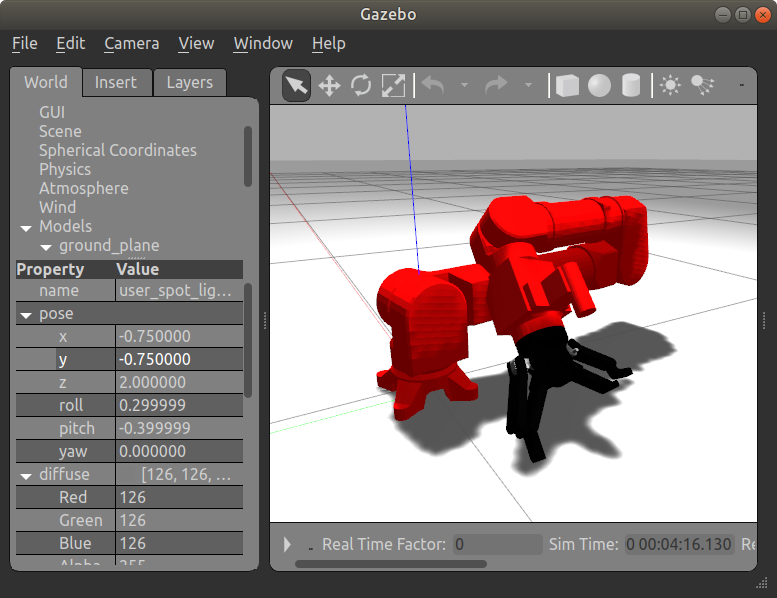
\includegraphics[width=\textwidth]{Figures/gazebo_ovis_sim.png}
    \caption{La pince Robotiq simulée avec Gazebo suite à une collision légère}
    \label{fig:robotiq_gazebo}
\end{figure}

Suite au développement de l'algorithme de contrôle du bras, il apparaît maintenant évident que le contrôle de la pince ne doit pas être intégré à celui-ci. Le contrôleur de la pince existant sera simplement lancé sur l'ordinateur embarqué de la plateforme mobile et le UI fera les appels nécessaires afin de contrôler manuellement l'ouverture/fermeture de la pince.
\chapter{Résultats et discussion}
Ce chapitre discute des résultats obtenus par ce projet.

\section{Description du bras robotique Ovis}
La définition du bras représente de manière fidèle le bras physique. Les membrures et joints sont positionnés adéquatement et leurs limites sont bien définies. La description est modulaire puisque la géométrie du bras est appelée à être modifiée au cours des prochaines années.

\section{Simulation}
\subsection{Simulateur industriel}
La simulation du manipulateur par le simulateur industriel est efficace pour effectuer le développement d'un algorithme. Toutefois, l'affichage des mouvement dans RViz est légèrement saccadé, ceci semble être un défaut provenant du simulateur industriel plutôt que de l'algorithme développé. Afin de valider cette hypothèse, un algorithme de contrôle préexistant fut testé et la simulation répondait de manière similaire.

\subsection{Simulateur Gazebo}
La simulation du manipulateur avec Gazebo est maintenant complété. Toutefois, la pince Robotiq apparaît mais n'est pas simulé adéquatement tel que mentionné à la section \ref{subsec:pince_gazebo}. L'ajout d'un contrôleur logiciel réglerait ce problème, mais puisqu'il n'y a pas de valeur ajoutée pour ce projet la pince restera simulée ainsi. La figure \ref{fig:gazebo_sim_rviz} montre la visualisation du bras dans RViz, lors de la simulation par Gazebo. On aperçoit l'image de la caméra au poignet aussi générée par Gazebo.
Une vidéo de la simulation est disponible en ligne à \url{https://youtu.be/ZcYvDAnuGzY}.

\begin{figure}
    \centering
    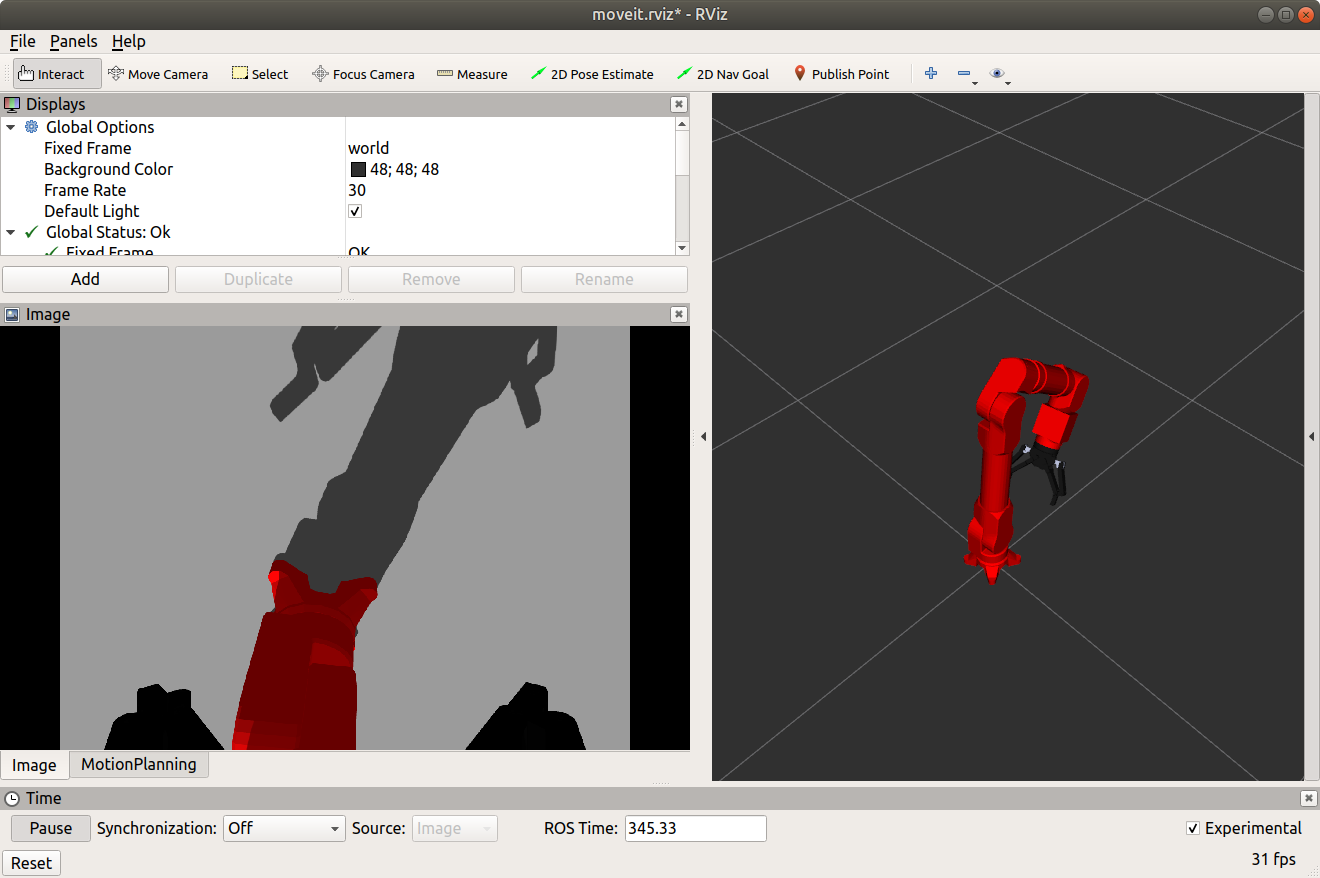
\includegraphics[%scale=0.35
                    width=\textwidth]{Figures/gazebo_sim_rviz.png}
    \caption{Ovis et sa caméra simulée par Gazebo et visualisée dans RViz}
    \label{fig:gazebo_sim_rviz}
\end{figure}


\section{Algorithme}
L'algorithme de contrôle en C++ est qualitativement plus rapide que le prototype précédent. Afin de valider que l'algorithme est, tel que souhaité, c'est à dire simple d'utilisation pour un opérateur n'ayant aucune expérience préalable, l'algorithme fut testé par quelques personnes externes au projet. Il n'y a eu aucun commentaires négatifs, l'expérience fut appréciée de tous. L'algorithme comporte toutefois certaines lacunes. Tout comme un robot industriel en mode \emph{jog} qui effectue un mouvement linéaire, lorsque deux axes se trouvent à être parallèles le bras arrive à une singularité. L'algorithme ne gère pas ce cas particulier. Aussi, lorsque la pince du robot approche la limite de la zone de travail, le robot peut être plus difficile à manipuler puisqu'il perd généralement %là-aussi 
un degré de liberté. Une solution envisagée pour palier ce problème est d'ajouter un contrôleur qui plutôt que de commander directement le système d'axes de référence, enverrait un vecteur afin de pousser/tirer virtuellement sur le système d'axes à l'outil. Finalement, malgré que l'algorithme permette au bras d'éviter les collisions avec lui-même et les objets connus de son environnement, celui-ci dépend de capteurs externes au bras. Une collision est possible entre le bras et un élément inconnu de l'environnement. Un événement de ce type n'est pas prévisible, mais l'algorithme pourrait être amélioré afin de tenir compte des capteurs de forces présent dans les actuateurs du bras et ainsi éviter d'endommager le manipulateur. En résumé, l'algorithme répond bien aux critères énoncés en début de projet et ce malgré qu'il ne soit fonctionnel que sur une plage réduite de l'enveloppe totale de travail accessible par le manipulateur.

\begin{figure}
    \centering
    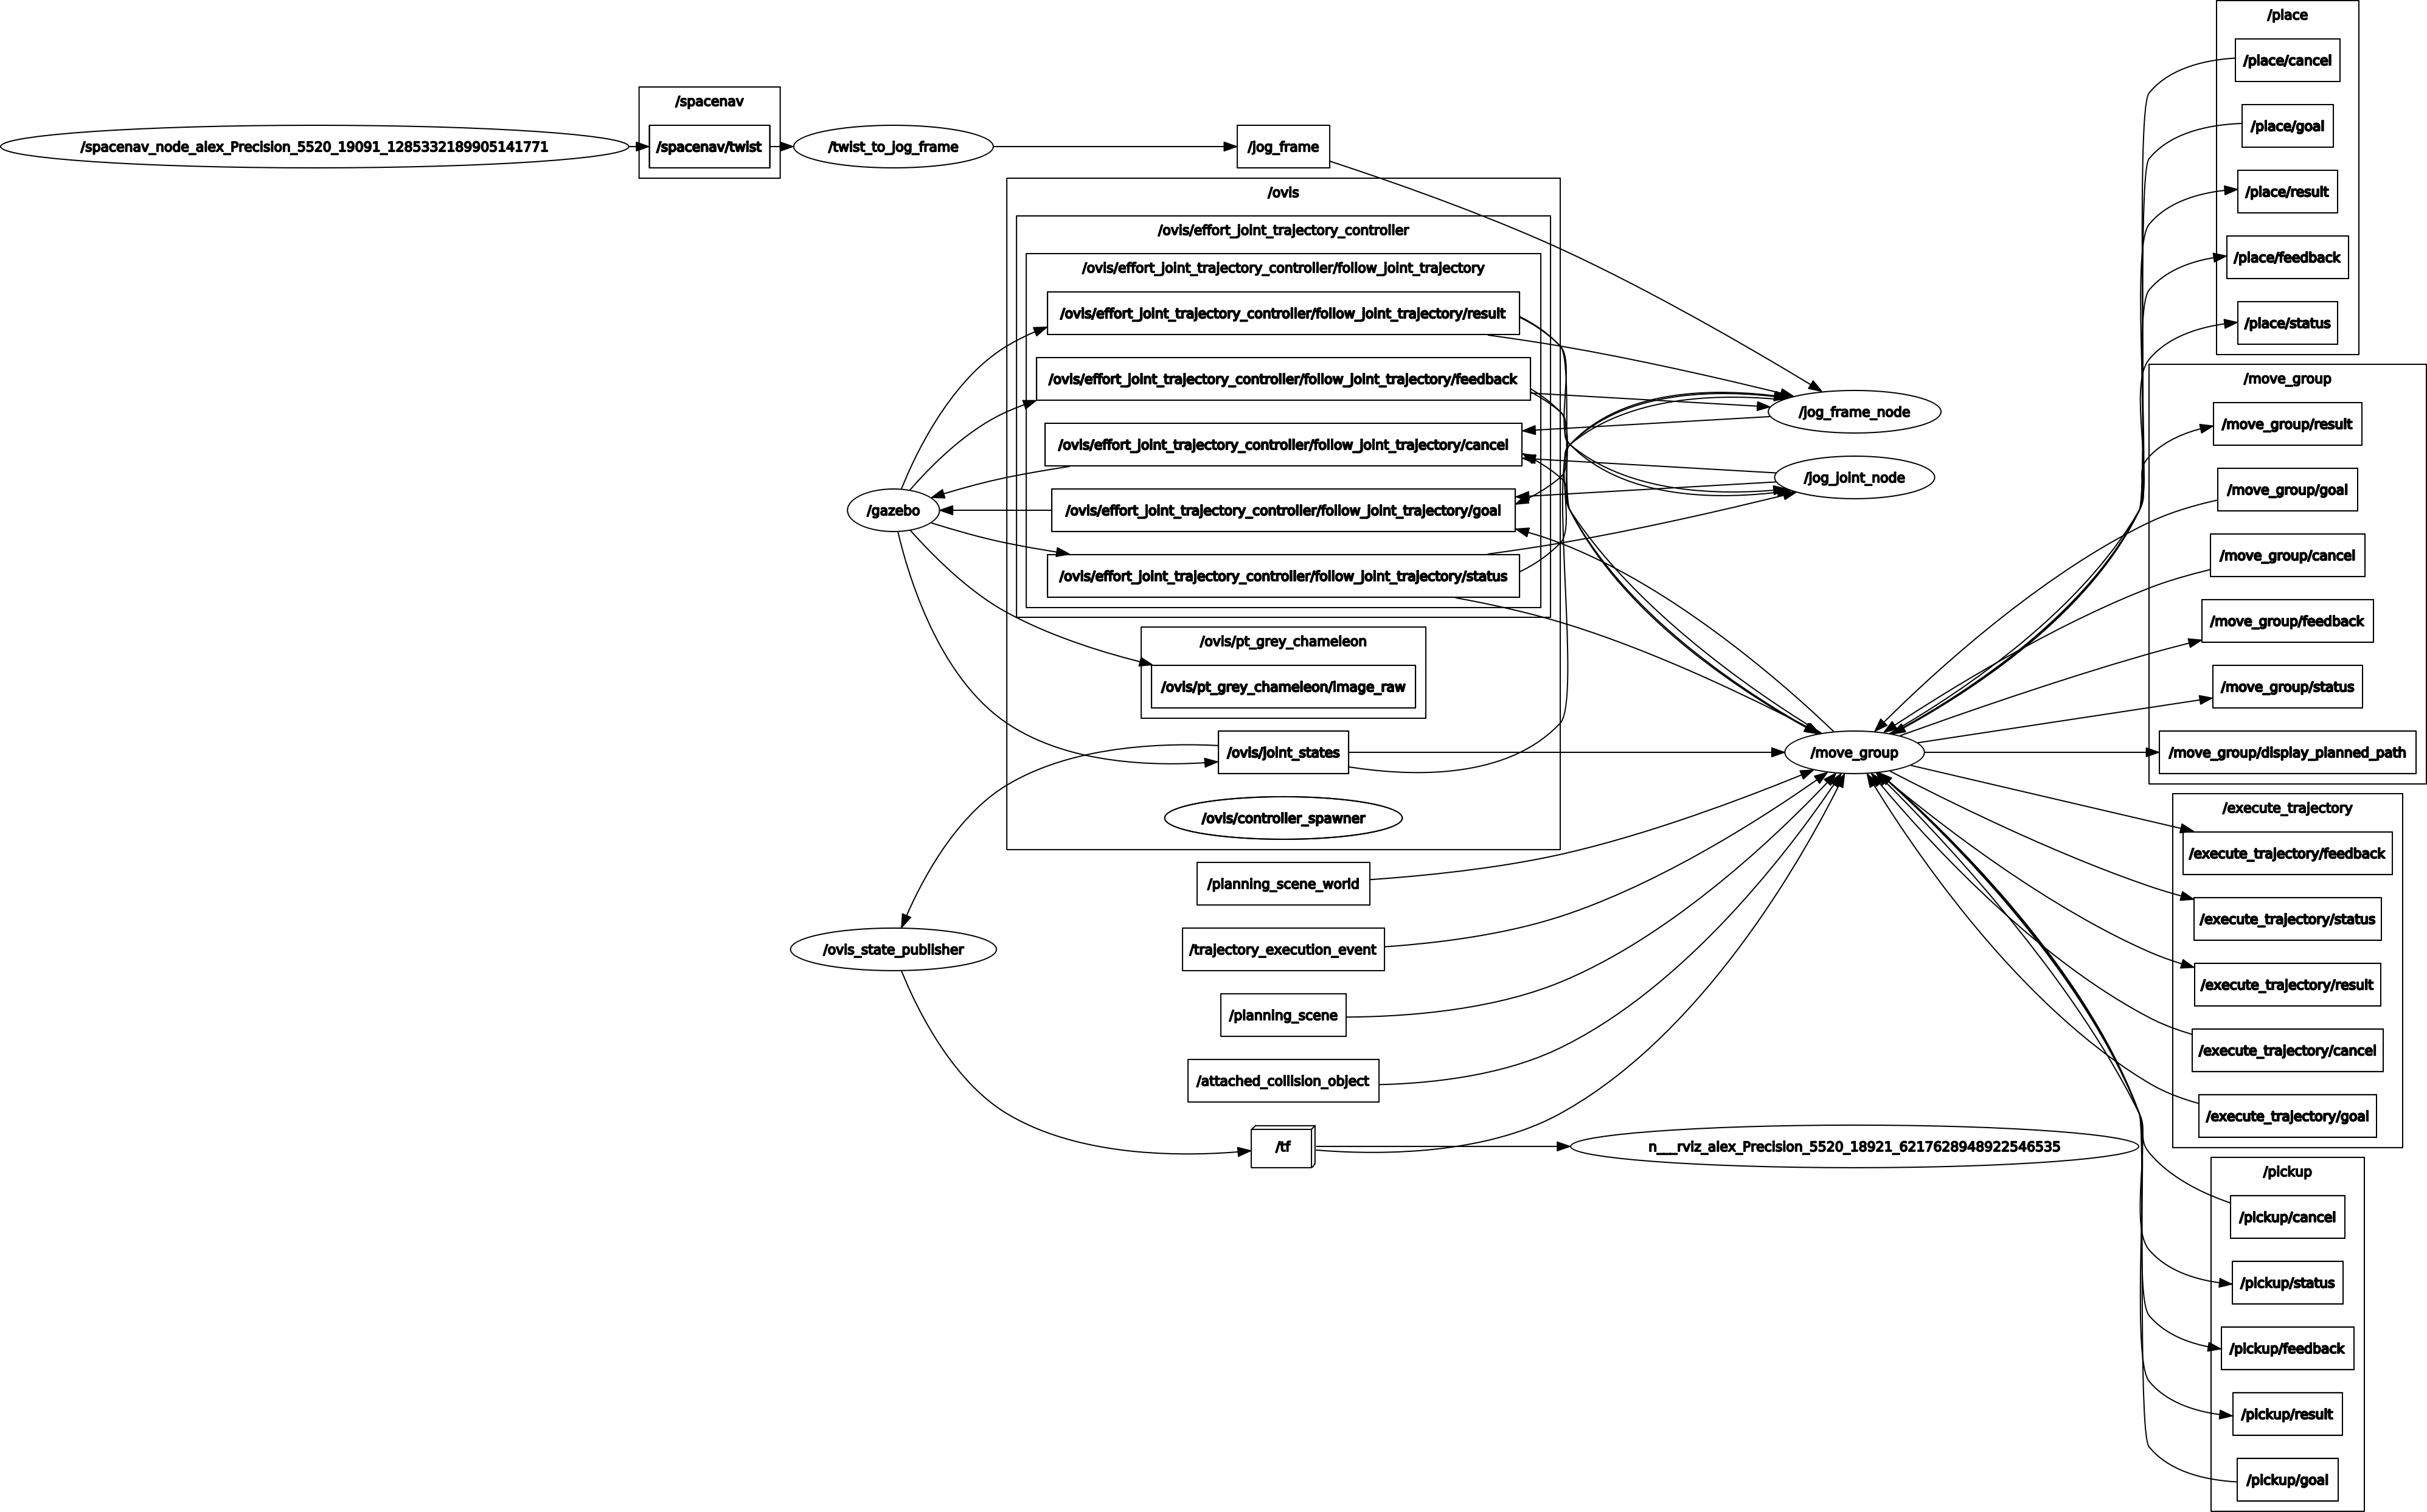
\includegraphics[%scale=0.35
                    width=\textwidth]{Figures/ovis_rosgraph_sim.png}
    \caption{Liaisons entre les différents noeuds logiciel de la solution}
    \label{fig:rosgraph_sim}
\end{figure}

\section{Interface matériel logiciel}
La communication entre le logiciel et le matériel n'est pas au point. L'ordinateur est apte à communiquer avec le contrôleur Kinova, ceci fut validé par l'envoi de commandes au travers du \emph{UI} fourni par Kinova. Toutefois, la communication entre le logiciel MoveIt et le contrôleur logiciel fourni par Kinova n'est pas complétée. Le contrôleur logiciel Kinova est détecté par le noeud ROS mais n'est pas détecté par MoveIt. Les causes possibles sont les suivantes: la connexion USB est instable, le nom de \emph{topic} attendu par MoveIt ne correspond pas à celui publié par le \emph{driver} Kinova. Ceci est une tâche de configuration assez ardue puisqu'il n'est pas évident à première vue d'établir tous les liens nécessaires. À titre d'exemple, la figure \ref{fig:rosgraph_sim} montre les liaisons entre les différents noeuds logiciel nécessaires au fonctionnement de la simulation visualisés à l'aide du logiciel rqt\_graph\footnote{\href{http://wiki.ros.org/rqt_graph}{wiki.ros.org/rqt\_graph}}. Malgré que ce point du projet est important pour la participation du club à la compétition. Il n'est pas critique à la validation de ce projet, la simulation étant suffisante à l'évaluation de l'algorithme. Il est important de mentionner que puisque l'algorithme est générique, celui-ci pourrait être testé sur tout autre robot supporté par ROS-Industrial et le logiciel \emph{jog\_control}.



%- Conclusion -%%
\begin{conclusion}
En guise de conclusion, ce projet montre qu'il est possible de contrôler un bras robotique à l'aide d'une souris 3D.
% Il est agréable de constater l'impact du logiciel libre, sans logiciels libres, ce projet n'aurait pas été réalisé dans d'aussi bref délais. 
Il aurait bien entendu été intéressant de réussir à établir la communication entre le logiciel et le matériel, mais la preuve de concept sur simulateur est suffisante en elle-même afin de déclarer ce projet un succès. 

Ce projet permis d'appliquer les notions apprises dans les cours GPA546 (Robots industriels) et GPA434 (Ingénierie des systèmes orientés objet). Il est important de mentionner que la matière du défunt cours GPA435 (Systèmes d'exploitation et programmation de systèmes) aurait fort probablement aidé à régler certains problèmes rencontrés au cours de ce projet puisque l'entièreté du logiciel développé ici repose sur Linux.

Dans le cadre d'une mission de recherche et sauvetage, l'algorithme développé par ce projet permettra à l'opérateur de sauver de précieuses minutes sur les manipulations. Malgré qu'elle n'ait pas été mesurée, la réduction de la charge mentale est flagrante par rapport au contrôle joint par joint. L'algorithme habilitera aussi l'opérateur à effectuer des manipulations préalablement impossible. Ce domaine étant lié au militaire, l'exemple le plus fréquent de manipulation sensible est la manipulation d'une bombe tuyau%\footnote{\href{https://en.wikipedia.org/wiki/Pipe_bomb}{wikipedia.org/wiki/Pipe\_bomb}}
. L'algorithme développé permettant de tirer dans un axe précis, ceci rend l'opération plus sécuritaire car il réduit le risque d'explosion soudaine et non contrôlée. 

En terminant, il serait éventuellement intéressant de comparer l'efficacité de l'algorithme développé dans le cadre de ce projet avec l'algorithme jog\_arm\footnote{\href{https://ros-planning.github.io/moveit_tutorials/doc/arm_jogging/arm_jogging_tutorial.html}{ros-planning.github.io/moveit\_tutorials/doc/arm\_jogging/arm\_jogging\_tutorial.html}} qui fut ajouté à la documentation officielle de MoveIt récemment.
\end{conclusion}

%%%%%%%%%%%%%%%%%%%%%%%%%%%%%%%%%%%%%%%%%%%%%%%%%%%
% Annexe
%%%%%%%%%%%%%%%%%%%%%%%%%%%%%%%%%%%%%%%%%%%%%%%%%%%
\appendix

%%%%%%%%%%%%%%%%%%%%%%%%%%%%%%%%%%%%%%%%%%%%%%%%%%%
% BIBLIOGRAPHIE ET RÉFÉRENCES
%%%%%%%%%%%%%%%%%%%%%%%%%%%%%%%%%%%%%%%%%%%%%%%%%%%

%%- Bibliographie -%%
\newpage
%Interligne sinmple pour la bibliographie
\begin{spacing}{1}
    % \nocite{*} % Utiliser la commande nocite pour afficher des références qui n'ont pas été citées dans le document. '*' permet de toutes les afficher.
	\bibliographystyle{bibETS} % Utilisation du style bibliographique de l'ETS
	\addcontentsline{toc}{chapter}{BIBLIOGRAPHIE} % Ajout de la bibliographie à la table des matières

% 	\bibliography{logiciel.bib} % Liste des fichiers bib de bibliographie, biblio.bib est un exemple
    \bibliography{Robots.bib}
\end{spacing}

%%- Références, exemple des références "refs" --%
%%%%%%%%%%%%%%%%%%%%%%%%%%%%%%%%%%%%%%%%%%%%%%%%%%%
% IMPORTANT: NOTES POUR COMPILER ET AFFICHER LES RÉFÉRENCES ADDITIONNELLES (remplacer "refs" par le suffixe choisi)
%%%%%%%%%%%%%%%%%%%%%%%%%%%%%%%%%%%%%%%%%%%%%%%%%%%
% Suivre les trois étapes:
%   1. Compiler le document une fois pour renseigner les références utilisées dans refs.aux
%   2. Lancer la compilation des références
% 		- Sous Linux: Utilser la commande "bibtex refs" dans le dossier du document
%		- Sous MacOSX (distribution MacTex): Utilser la commande "/usr/texbin/bibtex refs" dans le dossier du document
%		- Sous Windows: Éditer le script "update_refs.bat" pour renseigner le bon suffixe, et le lancer
%   3. Recompiler le document deux fois
%%%%%%%%%%%%%%%%%%%%%%%%%%%%%%%%%%%%%%%%%%%%%%%%%%%

% \newpage
% % Le fonctionnement est similaire, en rajoutant le suffixe choisi "refs" à la fin de chaque commande de bibliographie
% \begin{spacing}{1}
% 	%\nociterefs{*}
% 	\bibliographystylerefs{bibETS}
% 	\addcontentsline{toc}{chapter}{LISTE DE RÉFÉRENCES}

% 	\bibliographyrefs{refs} % Liste des fichiers bib de référence, refs.bib est un exemple

% \end{spacing}

% \chapter{Sources des références bibliographiques}
% \input{Texte/sourcesRef.tex}


% \input{Texte/carte_concept.tex}
\chapter{Robots actuellement sur le marché}\label{annexe:inspirationRobots}

\begin{figure}
    \centering
    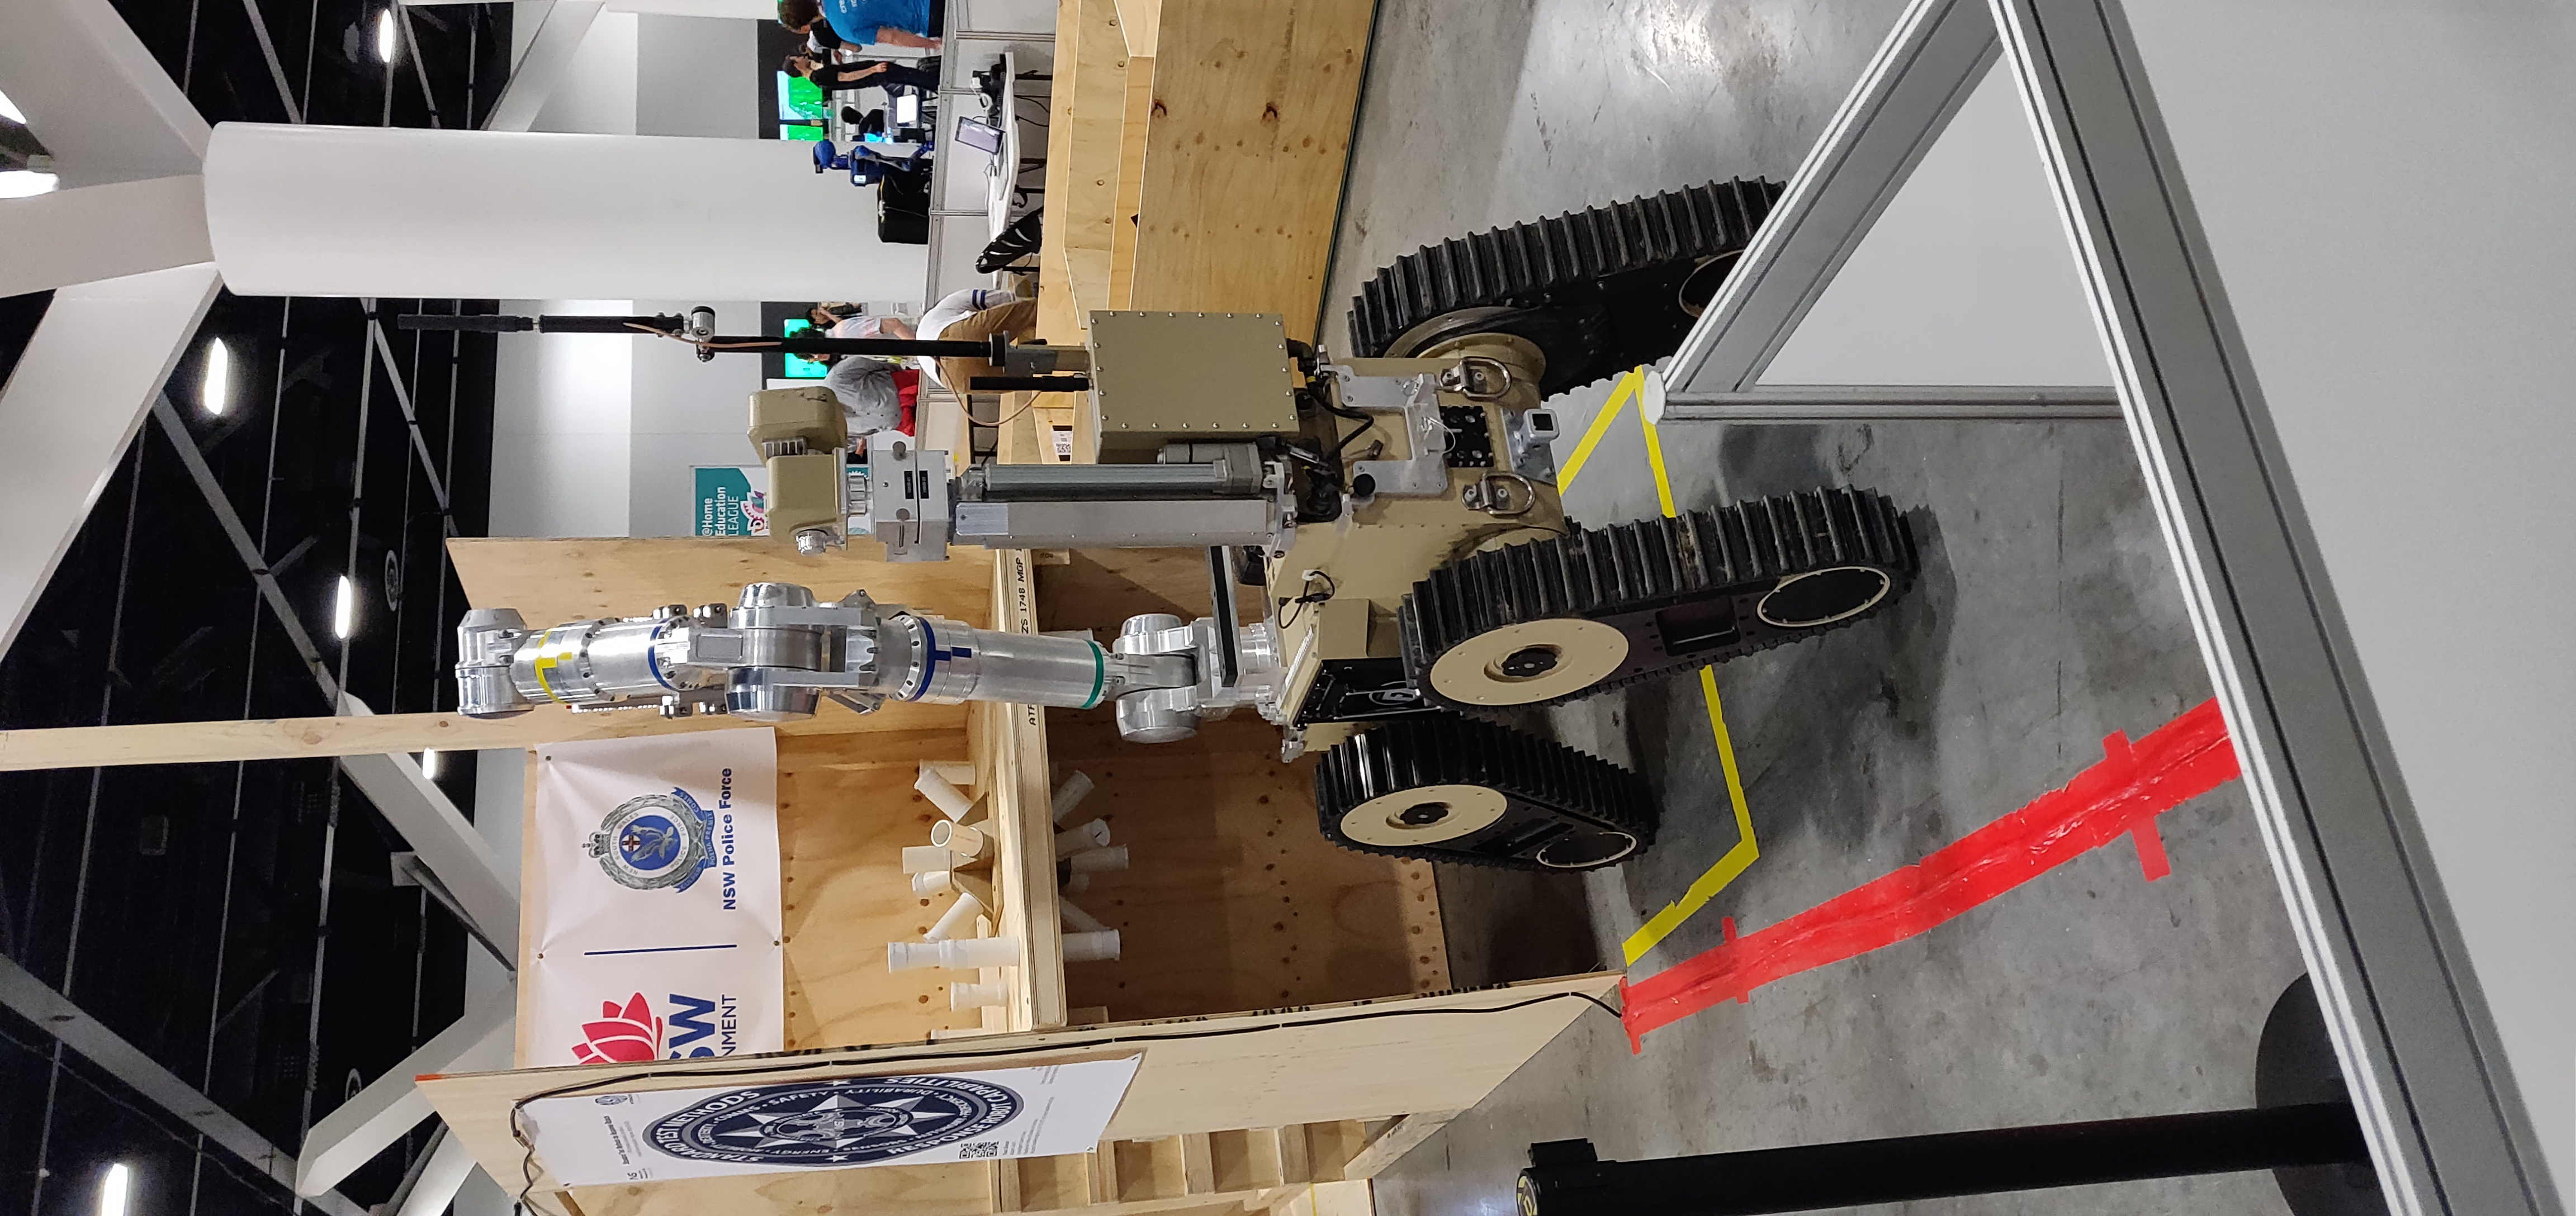
\includegraphics[width=0.55\textwidth, angle=270, origin=c, trim={25cm 0 35cm 0},clip=true]{Figures/andros.jpg}
    \caption{Northrop Grumman Remotec Andros}
    \label{fig:andros}
\end{figure}

\begin{figure}
    \centering
    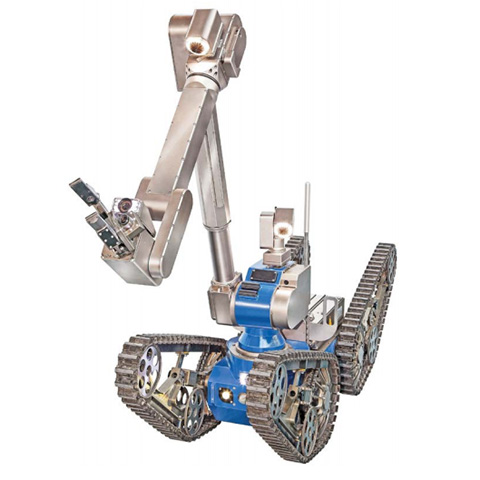
\includegraphics[width=0.5\textwidth]{Figures/telerob_telemax_PRO.jpg}
    \caption{Telerob telemax PRO}%\href{https://www.telerob.com/en/products/telemax-family/telemax-pro}
    \label{fig:telemaxPro}
\end{figure}
\end{document}